\documentclass[conference]{IEEEtran}
\usepackage[T1]{fontenc}
\usepackage[utf8]{inputenc}
\usepackage[brazilian]{babel}
\usepackage{cite}
\usepackage{amsmath,amssymb}
\usepackage{graphicx}
\usepackage{booktabs}
\usepackage{url}
\usepackage{xcolor}
\def\UrlBreaks{\do\/\do-\do.}

\begin{document}

\title{Um GPT para Machado de Assis: corpus, tokenização e transferência de aprendizado com o nanoGPT}

\author{\IEEEauthorblockN{Yan Tavares de Oliveira}
\IEEEauthorblockA{\textit{Departamento de Engenharia Elétrica}\\
\textit{Universidade de Brasília}\\
Brasília, Brasil\\
Matrícula: 252104296}}

\maketitle

\begin{abstract}
Este trabalho treina e avalia modelos de linguagem no estilo do GPT-2 sobre a obra completa de Machado de Assis, usando o nanoGPT como base. O corpus foi montado a partir dos 246 arquivos do acervo do Ministério da Educação: 243 obras e 13,4 milhões de caracteres depois da limpeza, com 99,1\% de cobertura em relação a uma segunda edição digital. Dez modelos e três linhas de base de n-gramas foram comparados em bits por caractere no mesmo conjunto de teste, métrica que independe do tokenizador. O GPorTuguese-2, versão do GPT-2 adaptada ao português, ajustado ao corpus atinge 1,369 bits por caractere, contra 1,530 do melhor modelo treinado só em Machado e 3,42 do bigrama. Com a mesma arquitetura, o tokenizador BPE português supera o de caracteres, e o GPT-2 pré-treinado em inglês, mesmo ajustado, fica atrás de um modelo de caracteres 11 vezes menor. O texto gerado reproduz vocabulário e marcas do estilo do autor sem copiar o treino, mas é menos variado que o texto real. Um protótipo de perguntas e respostas com recuperação de passagens encontra a obra certa entre as cinco primeiras passagens em 90\% das perguntas, e o gerador, treinado só para continuar texto, raramente converte a passagem em resposta, o que motiva o ajuste por instruções como próximo passo.
\end{abstract}

\begin{IEEEkeywords}
modelos de linguagem, Transformer, GPT-2, nanoGPT, Machado de Assis, tokenização, ajuste fino
\end{IEEEkeywords}

\section{Introdução}

Um modelo de linguagem autorregressivo estima a probabilidade de cada símbolo de um texto dado o que veio antes. A família GPT faz isso com a parte decodificadora do Transformer~\cite{vaswani2017attention} e mostrou que o mesmo objetivo, com mais parâmetros e mais dados, leva de modelos que completam frases a modelos que resolvem tarefas a partir de poucos exemplos no prompt~\cite{brown2020gpt3}. O nanoGPT~\cite{karpathy2022nanogpt} reimplementa o GPT-2 em PyTorch em dois arquivos de pouco mais de 300 linhas cada, um para o modelo e outro para o treino, e serve de base para este trabalho, junto com o código da aula em vídeo em que Karpathy constrói o modelo passo a passo~\cite{karpathy2023video}.

O problema tratado aqui é treinar e avaliar um modelo desse tipo na obra de Machado de Assis. O acervo inteiro, em domínio público, soma cerca de 13 milhões de caracteres depois de limpo: pouco para treinar um GPT-2 do zero e suficiente para ajustar um modelo pré-treinado. Três perguntas orientam os experimentos. Quanto se ganha ao passar dos n-gramas do início da aula para o Transformer? Tokenizar por caractere ou por subpalavra muda o resultado, e qual subpalavra? Pré-treinar em português antes de ver Machado ajuda mais do que aumentar o modelo treinado só no corpus?

As contribuições são: (i) um corpus limpo e validado da obra completa, com divisão treino/validação/teste que cobre todos os gêneros; (ii) uma comparação de dez modelos e três linhas de base na mesma métrica, bits por caractere, que independe do tokenizador; (iii) um protótipo de perguntas e respostas sobre as obras com recuperação de passagens, que mostra o que falta para o modelo responder perguntas.

\section{Fundamentação}

\subsection{Transformer decodificador}

Cada token $x_t$ vira a soma de um vetor de conteúdo e um vetor de posição. Um bloco do Transformer aplica atenção causal e depois uma rede densa por posição, ambas com conexão residual e normalização de camada. Na atenção, cada posição projeta consultas $Q$, chaves $K$ e valores $V$ e combina os valores das posições anteriores com pesos
\begin{equation}
\text{Atenção}(Q,K,V)=\mathrm{softmax}\!\left(\frac{QK^\top}{\sqrt{d_k}}+M\right)V,
\end{equation}
em que $M$ vale $-\infty$ acima da diagonal, para que nenhuma posição veja o futuro, e a divisão por $\sqrt{d_k}$ evita que o softmax sature~\cite{vaswani2017attention}. Várias cabeças fazem isso em paralelo sobre subespaços de dimensão $d_k=d/h$. O GPT-2, na implementação do nanoGPT~\cite{karpathy2022nanogpt}, põe a normalização antes de cada subcamada, usa GELU na rede densa e compartilha a matriz de embeddings com a camada de saída.

\subsection{Objetivo e métrica}

O treino minimiza a entropia cruzada média $\mathcal{L}=-\frac{1}{N}\sum_t \log p_\theta(x_t\mid x_{<t})$ em nats por token. Essa perda não se compara entre tokenizadores, porque um token de caractere e um token BPE cobrem quantidades diferentes de texto. Por isso todos os modelos são avaliados em bits por caractere,
\begin{equation}
\mathrm{bpc}=\frac{\sum_t -\log p_\theta(x_t\mid x_{<t})}{C\,\ln 2},
\end{equation}
em que a soma percorre todos os tokens do conjunto de teste e $C$ é o número de caracteres que eles codificam. A perplexidade por palavra, $\exp(\sum_t -\log p_\theta/W)$ com $W$ palavras, tem a mesma propriedade.

\subsection{Escala e transferência}

Brown et al.~\cite{brown2020gpt3} treinaram o GPT-3, com 175 bilhões de parâmetros e 300 bilhões de tokens, e mostraram que a perda cai de forma regular com a computação e que o modelo resolve tarefas novas a partir de alguns exemplos no prompt, sem ajuste de pesos. O corpus de Machado tem de 3 a 5 milhões de tokens BPE, conforme o tokenizador, cinco ordens de grandeza abaixo. A saída usual para corpora pequenos é a transferência: partir de um modelo pré-treinado em muito texto e ajustá-lo ao domínio, como no exemplo de ajuste fino do nanoGPT~\cite{karpathy2022nanogpt}. O GPorTuguese-2\footnote{\url{https://huggingface.co/pierreguillou/gpt2-small-portuguese}} é o GPT-2 small (124M parâmetros) ajustado em 1,28~GB da Wikipédia em português, com um vocabulário BPE próprio, diferente do original.

\section{Corpus}

\subsection{Fonte e limpeza}

A fonte é a Obra Completa publicada pelo Ministério da Educação em \url{http://machado.mec.gov.br}, redistribuída como corpus \texttt{machado} do NLTK: 246 arquivos em oito gêneros. A limpeza é feita pelo script \texttt{corpus.py}.

Os arquivos estão em Windows-1252. Lidos como Latin-1, o travessão dos diálogos (byte 0x97) vira um caractere de controle invisível e a marca de fala desaparece do corpus inteiro. Parte dos arquivos grafa o travessão como ``\texttt{-{}-}'', e as duas formas foram unificadas. As linhas quebram na largura de coluna do arquivo; as quebras dentro de cada parágrafo foram desfeitas, e cada parágrafo (ou verso) passou a ocupar uma linha, para que o modelo aprenda a quebra de parágrafo e não a largura da página.

Do texto saíram o cabeçalho editorial de cada arquivo (gênero, edição de referência, ``Publicado originalmente\ldots'') e 45 índices. Um índice termina quando uma de suas entradas reaparece como título no texto; em 5 dos 45 isso não acontece, e o índice termina no primeiro parágrafo longo. Havia 123 parágrafos longos repetidos: 99 entre arquivos (críticas republicadas, crônicas presentes em duas coletâneas e dois contos que compartilham trechos) e 24 dentro do mesmo arquivo. Cada um ficou só na primeira ocorrência, para não aparecer ao mesmo tempo no treino e no teste. As três traduções (de Dickens, de Victor Hugo e de Girardin e Dumas Filho) foram excluídas, porque não são prosa original de Machado.

O resultado, \texttt{machado\_obra\_completa.txt}, tem 243 obras, 13,39 milhões de caracteres, 2,36 milhões de palavras e 144 caracteres distintos. Os contos respondem por 39\% do texto, a crônica e o romance por 23\% cada, a crítica por 7\%, a poesia por 5\% e o teatro por 3\%.

\subsection{Validação e divisão}

Para verificar se a limpeza descartou texto literário, o corpus foi comparado a uma segunda edição digital das mesmas obras, extraída de PDFs. De todos os 8-gramas de palavras dessa edição, 99,1\% aparecem no corpus limpo (97,0\% na poesia, provavelmente porque a disposição dos versos difere entre as edições). Nas traduções, excluídas, a cobertura é zero, como esperado.

O texto de cada obra foi cortado em blocos de cerca de 4.000 caracteres, numerados em sequência ao longo de todo o acervo. De cada 20 blocos, 18 vão para o treino, um para a validação e um para o teste. Assim os três conjuntos cobrem todos os gêneros e épocas, e nenhum trecho contínuo aparece em dois deles. O treino tem 12,04 milhões de caracteres; validação e teste têm 0,68 milhão cada.

\subsection{Tokenização}

O mesmo texto foi codificado de três formas: por caractere (vocabulário de 144 símbolos, como no vídeo), com o BPE do GPT-2 (50.257 tokens aprendidos em texto em inglês) e com o BPE do GPorTuguese-2 (também 50.257 tokens, com vocabulário próprio). O BPE inglês produz 2,53 caracteres por token no corpus, contra 4,01 do BPE português: ``coração'', por exemplo, vira quatro tokens no primeiro e um no segundo. Com o mesmo contexto de 512 tokens, o modelo português enxerga 58\% mais texto. Nos três casos a decodificação reproduz o texto original sem perda, condição para o cálculo do bpc.

\section{Metodologia}

\subsection{Modelos}

Todos os modelos treinados por gradiente têm a arquitetura do GPT-2 implementada no \texttt{model.py} do nanoGPT, exceto o GPT do vídeo, que usa o código da aula~\cite{karpathy2023video}. A Tabela~\ref{tab:resultados} lista tamanhos e contextos. Os experimentos formam quatro grupos.

\emph{Linhas de base.} Unigrama, bigrama e trigrama de caracteres, estimados por contagem com suavização aditiva escolhida na validação. O primeiro modelo do vídeo é um bigrama neural, que no ótimo coincide com o bigrama de contagens sem suavização.

\emph{Caracteres, do zero.} Um modelo de 0,8M de parâmetros com a receita de CPU do README do nanoGPT (4 camadas, 128 dimensões, contexto de 64), treinado na CPU; o ``baby GPT'' de 10,8M (6 camadas, 6 cabeças, 384 dimensões, contexto de 256) com a configuração \texttt{train\_shakespeare\_char} do nanoGPT; e um modelo de 25M (8 camadas, 512 dimensões, contexto de 512). O GPT do vídeo tem o mesmo tamanho do baby GPT e mantém o código da aula: atenção com um laço por cabeça, ReLU, sem compartilhamento de pesos, AdamW com taxa constante de $3\times10^{-4}$ e precisão fp32. A comparação entre os dois mede o efeito conjunto das escolhas de engenharia do nanoGPT (GELU, inicialização escalada, pesos compartilhados, decaimento de peso seletivo, taxa maior com aquecimento e decaimento cosseno, recorte de gradiente, atenção fundida e fp16).

\emph{BPE, do zero.} A arquitetura do baby GPT com os tokenizadores BPE inglês e português (vocabulário de 50.257, contexto de 256 tokens), para medir o efeito do tokenizador sem pré-treino.

\emph{Pré-treinados.} GPT-2 small e GPorTuguese-2 (124M), avaliados sem nenhum treino no corpus (zero-shot) e ajustados por 1.200 iterações com contexto de 512 tokens, lotes de 16.384 tokens, taxa máxima de $6\times10^{-5}$ com decaimento cosseno e dropout de 0,1, adaptando o exemplo de ajuste fino do nanoGPT (que usa taxa constante).

\subsection{Treino e avaliação}

Os modelos do nanoGPT usam AdamW com $\beta_2=0{,}99$ para modelos pequenos, recorte de gradiente em 1,0 e \texttt{torch.compile}, numa GPU NVIDIA T4 do Google Colab em fp16; a exceção é o modelo de 0,8M, treinado na CPU em fp32. O checkpoint mantido é o de menor perda de validação. A avaliação final percorre o conjunto de teste inteiro com janela deslizante: a primeira janela pontua todas as posições e as seguintes avançam meio contexto e pontuam só as posições novas, de modo que cada token é previsto uma vez e quase todos com pelo menos meio contexto. O mesmo cálculo é feito separadamente para o teste de cada gênero.

A qualidade do texto gerado é medida em 30 continuações de 400 caracteres por modelo (dez inícios de parágrafo sorteados do teste, três amostras cada, temperatura 0,8 e top-$k$ 200, os padrões do \texttt{sample.py}). As métricas são a fração de palavras que existem no vocabulário do treino, distinct-2 (bigramas de palavras distintos sobre o total), a fração de 8-gramas de palavras copiados literalmente do treino e a fração de 4-gramas repetidos dentro da própria amostra. As mesmas métricas, calculadas na continuação real de cada parágrafo, servem de referência.

\section{Resultados}

\begin{table*}[t]
\centering
\caption{Modelos e resultados no conjunto de teste (677 mil caracteres). Parâmetros em milhões; contexto em tokens; tempo de treino em minutos numa GPU T4 (o modelo de 0,8M foi treinado na CPU). A perplexidade por palavra usa o mesmo total de log-verossimilhança do bpc. Em negrito, o melhor resultado.}
\label{tab:resultados}
\footnotesize
\begin{tabular}{lccccccc}
\toprule
Modelo & Tokens & Parâm. (M) & Contexto & Inicialização & Treino (min) & bpc teste & Perpl. palavra \\
\midrule
Unigrama & char & -- & -- & contagem & -- & 4,470 & -- \\
Bigrama (vídeo) & char & -- & -- & contagem & -- & 3,422 & -- \\
Trigrama & char & -- & -- & contagem & -- & 2,860 & -- \\
Char 0,8M (CPU) & char & 0,8 & 64 & aleatório & 2 & 2,691 & 40.260 \\
GPT do vídeo 10,8M & char & 10,8 & 256 & aleatório & 52 & 1,725 & 894 \\
nanoGPT char 10,8M & char & 10,8 & 256 & aleatório & 13 & 1,632 & 621 \\
nanoGPT char 25M & char & 25,5 & 512 & aleatório & 30 & 1,565 & 478 \\
BPE GPT-2, do zero & BPE en & 30,0 & 256 & aleatório & 17 & 1,574 & 494 \\
BPE pt, do zero & BPE pt & 30,0 & 256 & aleatório & 17 & 1,530 & 415 \\
GPT-2 124M zero-shot & BPE en & 124,0 & 512 & GPT-2 & 0 & 2,804 & 63.001 \\
GPorTuguese-2 zero-shot & BPE pt & 124,0 & 512 & GPorT.-2 & 0 & 1,593 & 532 \\
GPT-2 124M ajustado & BPE en & 124,0 & 512 & GPT-2 & 29 & 1,723 & 889 \\
GPorTuguese-2 ajustado & BPE pt & 124,0 & 512 & GPorT.-2 & 28 & \textbf{1,369} & 220 \\
\bottomrule

\end{tabular}
\end{table*}

A Tabela~\ref{tab:resultados} e a Fig.~\ref{fig:bpc} resumem a comparação. O melhor modelo é o GPorTuguese-2 ajustado, com 1,369 bpc no teste, 11\% abaixo dos 1,530 do melhor modelo treinado só no corpus de Machado, e perplexidade de 220 por palavra.

\subsection{Do bigrama ao Transformer}

O bigrama, primeiro modelo do vídeo, fica em 3,42 bpc, e o trigrama em 2,86. O menor Transformer (0,8M de parâmetros, contexto de 64 caracteres, 2.000 iterações em 1,6 minuto na CPU) já passa o trigrama, com 2,69 bpc. O baby GPT, com 10,8M de parâmetros e contexto de 256, cai para 1,632 bpc em 13 minutos na T4. O GPT do vídeo, com o mesmo tamanho e os mesmos dados, fica em 1,725 bpc depois de 52 minutos de treino. O experimento não isola cada escolha de engenharia: a diferença de tempo vem provavelmente do fp32 e do laço por cabeça de atenção, e a de qualidade pode vir da taxa de aprendizado (constante em $3\times10^{-4}$ no vídeo, com pico de $10^{-3}$ e decaimento no nanoGPT) e da inicialização. Aumentar o modelo de caracteres para 25M de parâmetros e o contexto para 512 leva a 1,565 bpc.

\subsection{Tokenizador}

Com a mesma arquitetura do baby GPT e sem pré-treino, trocar caracteres pelo BPE português reduz o bpc de 1,632 para 1,530, e o BPE inglês, para 1,574. Os modelos BPE têm 30M de parâmetros, 19M deles na matriz de embeddings. O BPE português supera também o modelo de caracteres de 25M (1,565), e o inglês fica praticamente empatado com ele. O BPE português cobre 4,0 caracteres por token, e o contexto de 256 tokens alcança cerca de mil caracteres, quatro vezes o do modelo de caracteres. O preço é o sobreajuste: com 3 milhões de tokens de treino, as 3.000 iterações somam cerca de 16 épocas, e a perda de treino do BPE português (3,46 nats por token) fica bem abaixo da de validação (4,28).

\subsection{Pré-treino e ajuste fino}

O GPT-2 original, treinado em inglês, faz 2,80 bpc sem ajuste, pouco melhor que o trigrama (2,86). Só 64\% das palavras que ele gera existem no vocabulário de Machado, e algumas amostras passam ao inglês e entram em laço. O GPorTuguese-2 sem ajuste já faz 1,593 bpc, melhor que o baby GPT treinado no corpus, mas escreve num registro contemporâneo (``Eu estava tipo, malandro''). O ajuste fino por 1.200 iterações (28 minutos) leva esse modelo a 1,369 bpc. O mesmo ajuste no GPT-2 inglês chega a 1,723 bpc: com o tokenizador inglês e sem ter visto português, 124M de parâmetros rendem menos que 10,8M treinados por caractere. Nos dois ajustes a melhor validação está na última avaliação (Fig.~\ref{fig:curvas}); no GPT-2 a curva ainda descia, e no GPorTuguese-2 já estava quase plana desde a iteração 800.

\subsection{Gêneros}

A poesia é o gênero mais difícil para todos os modelos (Fig.~\ref{fig:generos}): 1,97 bpc no baby GPT e 1,82 no melhor modelo, contra 1,30 a 1,45 dos demais gêneros no modelo ajustado. A poesia é só 5\% do treino, e os versos, com vocabulário raro e ordem de palavras pouco usual, são provavelmente mais difíceis de prever. O ajuste fino do GPorTuguese-2 ganha mais no romance ($-0{,}26$ bpc em relação ao modelo sem ajuste) e no conto ($-0{,}24$) do que na crítica ($-0{,}14$), provavelmente porque a prosa ensaística se parece mais com a da Wikipédia do que o diálogo de ficção.

\subsection{Texto gerado}

A Tabela~\ref{tab:texto} mede as amostras. A partir do baby GPT, os modelos treinados ou ajustados no corpus escrevem de 97,8\% a 99,5\% de palavras existentes no vocabulário de Machado, patamar do próprio texto real (98,4\%). No texto real, as palavras ausentes do vocabulário são formas verbais raras (``devorais'', ``alimpais'') e palavras cortadas no limite de 400 caracteres, corte que também afeta as amostras. Nenhum modelo copiou trechos longos: a fração de 8-gramas presentes no treino é zero em todos, contra 0,6\% no texto real, em que o próprio Machado repete uma frase em duas crônicas (``que quer o senhor que eu faça com este câmbio'', com a cotação a 8 numa e a 9 na outra). A diversidade é o ponto fraco. O distinct-2 do texto real é 0,965, e o dos modelos a partir do baby GPT fica entre 0,78 e 0,87; o modelo de 0,8M chega a 0,94, provavelmente porque inventa palavras, que raramente se repetem. Entre os modelos treinados ou ajustados, a fração de 4-gramas repetidos dentro da amostra chega a 1,2\% (GPT-2 ajustado), contra 0,5\% no texto real. O exemplo abaixo mostra o início de uma amostra do GPorTuguese-2 ajustado a partir de um prompt fora do corpus:

\begin{quote}\small
\emph{Capitu olhou para mim}. Podia-lhe ver se eu não mandasse logo.\\
--- Dá-te-á lá, pensou eu; vou.\\
--- Mas não diga nada.\\
--- Não diga nada.\\
--- Mamãe quer falar-lhe?\\
--- Não fala, respondeu o cunhado.
\end{quote}

\noindent O diálogo tem o travessão, a mesóclise e o tratamento da época, mas não segue uma cena coerente. Na mesma amostra, cinco de 18 falas giram em torno de ``não diga'', ``não digo'' ou ``não me digo'', e uma fala se repete em seguida (``--- De queres?'').

\begin{figure}[t]
\centering
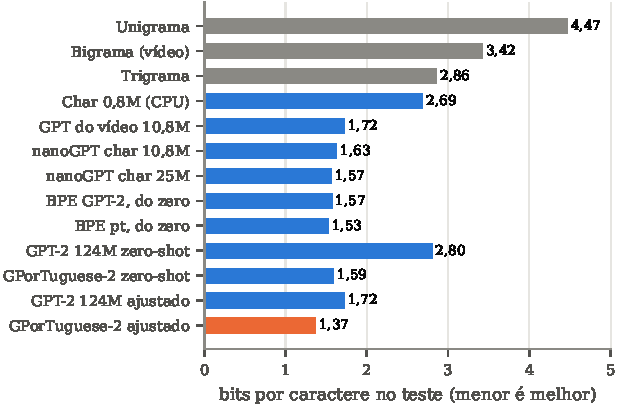
\includegraphics[width=\columnwidth]{figuras/bpc_teste.pdf}
\caption{Bits por caractere no teste. Cinza: n-gramas de contagem; azul: redes; laranja: melhor modelo.}
\label{fig:bpc}
\end{figure}

\begin{figure*}[t]
\centering
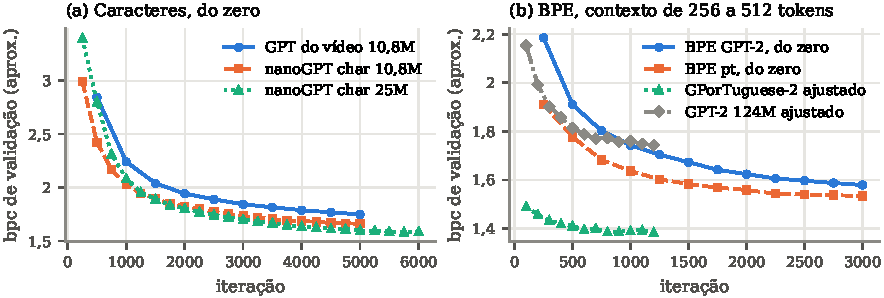
\includegraphics[width=\textwidth]{figuras/curvas.pdf}
\caption{Validação ao longo do treino, convertida de nats por token para bpc pela razão média de caracteres por token de cada tokenizador. A estimativa usa lotes aleatórios do \texttt{train.py} e fica um pouco acima do bpc exato de teste.}
\label{fig:curvas}
\end{figure*}

\begin{figure}[t]
\centering
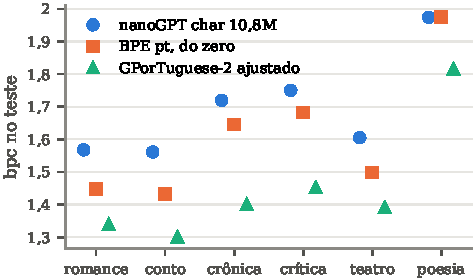
\includegraphics[width=\columnwidth]{figuras/generos.pdf}
\caption{Bits por caractere no teste de cada gênero (miscelânea omitida: 4 mil caracteres).}
\label{fig:generos}
\end{figure}

\begin{table}[t]
\centering
\caption{Qualidade de 30 continuações de 400 caracteres por modelo, em \%, exceto distinct-2. Válidas: palavras presentes no vocabulário do treino; memor.: 8-gramas copiados do treino; repet.: 4-gramas repetidos na amostra.}
\label{tab:texto}
\footnotesize
\setlength{\tabcolsep}{3pt}
\begin{tabular}{lcccc}
\toprule
Modelo & Válidas & distinct-2 & Memor. & Repet. \\
\midrule
Char 0,8M (CPU) & 61,4 & 0,937 & 0,0 & 0,0 \\
GPT do vídeo 10,8M & 97,8 & 0,851 & 0,0 & 0,0 \\
nanoGPT char 10,8M & 98,7 & 0,858 & 0,0 & 0,0 \\
nanoGPT char 25M & 98,3 & 0,871 & 0,0 & 0,0 \\
BPE GPT-2, do zero & 98,8 & 0,853 & 0,0 & 0,0 \\
BPE pt, do zero & 99,3 & 0,842 & 0,0 & 0,2 \\
GPT-2 124M zero-shot & 64,3 & 0,862 & 0,0 & 2,4 \\
GPorTuguese-2 zero-shot & 96,2 & 0,846 & 0,0 & 0,8 \\
GPT-2 124M ajustado & 98,2 & 0,783 & 0,0 & 1,2 \\
GPorTuguese-2 ajustado & 99,5 & 0,820 & 0,0 & 0,9 \\
\midrule
Texto real (teste) & 98,4 & 0,965 & 0,6 & 0,5 \\
\bottomrule

\end{tabular}
\end{table}


\section{Extensão: perguntas sobre o universo machadiano}

Os modelos deste trabalho aprenderam a continuar texto. Perguntado ``Quem era o melhor amigo de Bentinho no seminário?'', o GPorTuguese-2 ajustado responde ``--- Um amigo de meu pai.'', uma fala plausível de personagem e não a resposta (Escobar): nada no objetivo de treino liga uma pergunta a um fato das obras, e o conhecimento que ele tem de enredos e personagens está espalhado nos pesos, sem fonte que se possa conferir. Com 124M de parâmetros, a memória factual do modelo também é pequena~\cite{brown2020gpt3}.

Um caminho direto é a geração aumentada por recuperação: buscar no corpus as passagens relevantes e colocá-las no prompt, com a referência da obra, para que a resposta se apoie num trecho verificável. O protótipo \texttt{rag.py} corta as 243 obras em passagens de cerca de 600 caracteres e as indexa por TF-IDF de unigramas e bigramas de palavras. Num conjunto de 20 perguntas com resposta conhecida (personagens, lugares e ideias de romances e contos), escritas sem a palavra da resposta, a palavra da resposta aparece em alguma das cinco primeiras passagens em 70\% dos casos (35\% na primeira), e a obra certa em 90\% (70\% na primeira).

Os erros de recuperação mostram o que melhorar. Perguntas parafraseadas não compartilham palavras com o trecho certo (``posto militar'' contra ``alferes'', em \emph{O Espelho}). Além disso, contos publicados em coletânea são citados com o título do volume, e não do conto. Embeddings densos de sentenças em português devem reduzir o primeiro problema, e um índice por conto e capítulo, o segundo.

No protótipo, as três primeiras passagens (até 1.400 caracteres) entram no prompt do GPorTuguese-2 ajustado, seguidas de ``Pergunta: \ldots{} Resposta:''. Em 8 das 20 perguntas a palavra da resposta estava no prompt, e o modelo a usou uma vez (``Não, senhor; é o Dr. Simão Bacamarte''). Nas outras, respondeu como uma personagem (``Não, senhor; não é possível\ldots''), provavelmente porque no corpus pergunta e resposta só aparecem como diálogo. O passo seguinte é o ajuste por instruções: montar pares de pergunta e resposta ancorados em passagens do corpus (escritos à mão ou gerados por um modelo maior e revisados) e ajustar o modelo nesse formato. Para perguntas de relação (``quem é a madrasta de Iaiá Garcia?''), um grafo de personagens, obras e relações extraído do texto permite consultas exatas e serve de fonte para os próprios pares de treino. Em escala maior, um modelo pré-treinado em português com bilhões de parâmetros, combinado à mesma recuperação, trataria as perguntas analíticas (temas, narrador não confiável, ironia), deixando para o modelo pequeno o papel de gerar texto no estilo do autor. A avaliação pediria um conjunto de perguntas com respostas de referência revisadas por especialistas em Machado, medindo acerto da resposta e a fidelidade à passagem citada.

\section{Conclusão}

Este trabalho montou um corpus limpo e validado da obra completa de Machado de Assis e comparou, na mesma métrica, modelos do bigrama do vídeo ao GPT-2 ajustado. Com o mesmo corpo de Transformer do baby GPT, o BPE português reduz o bpc mais do que passar o modelo de caracteres de 10,8M para 25M de parâmetros (1,530 contra 1,565). O maior ganho vem do pré-treino no idioma certo: o GPorTuguese-2 ajustado chega a 1,369 bpc, enquanto o GPT-2 inglês, mesmo com 124M de parâmetros e o mesmo ajuste, fica atrás de um modelo de caracteres 11 vezes menor. Os modelos ajustados reproduzem a superfície do estilo (palavras válidas, travessão, mesóclise), mas geram texto menos variado que o real e não sustentam uma cena.

As principais limitações são o treino curto de vários modelos (a validação ainda caía no fim), uma única semente por configuração e a avaliação do texto gerado por métricas automáticas, sem leitores humanos. Para responder perguntas sobre as obras, o caminho proposto combina recuperação de passagens com ajuste por instruções; o protótipo mostra que a recuperação já encontra a obra certa na maioria dos casos e que o gerador, treinado só para continuar texto, ainda não transforma a passagem em resposta.

\section*{Disponibilidade do código}

O código, com as partes de terceiros (nanoGPT e código do vídeo, de A. Karpathy, licença MIT) separadas e marcadas, está no notebook do projeto e no repositório que o acompanha. As duas alterações feitas no nanoGPT estão isoladas em um patch.

\bibliographystyle{IEEEtran}
\bibliography{referencias}

\end{document}
